% !TeX root = vpl.tex

\chap{A Pet Robot}\label{ch.pet}

The robots we build in this chapter are called \emph{autonomous robots}.
They display independent behavior that is normally associated with
living things like cats and dogs. The behavior is achieved by
\textit{feedback}: the robot will sense that something occurs in the
world and modify its behavior accordingly.

\sect{The robot obeys you}

First, we will program the robot to obey. Normally, the robot stays in
place without moving; when it detects your hand in front of it, it
moves towards your hand.

There are five horizontal distance sensors on the front of the Thymio
robot and two on the rear of the robot.
They are similar to the ones under Thymio that we have used in \cref{ch.moving}.
%\footnote{The technical term is \emph{proximity sensor}, but we will use the simpler term \emph{horizontal distance sensor}.}
Bring your hand slowly towards the
sensors; when it gets close, a red light will appear around the sensors
that detect your hands (\cref{fig.detect}).

\begin{figure}
\begin{center}
\gr{detect}{.6}
\caption{The front of the Thymio. Two sensors detect the fingers.}\label{fig.detect}
\end{center}
\end{figure}

The block \blksm{event-prox} is used to sense if something is close to the
sensor or not. In either case it causes an event to occur. The small
gray squares (five on the front and two on the rear) are used to specify
when an event occurs. Clicking on a square changes it from gray to
white to red and back to gray.
For this block, the meaning of these colors is:

\begin{itemize}
\item \textbf{Gray}: The value of the sensor does not influence the
program.
\item \textbf{Red}: An event occurs when the sensor detects an object
close to it.
\item \textbf{White}: An event occurs when the sensor detects that there
is \emph{no} object nearby.
\end{itemize}

\importantbox[Ground sensors and horizontal sensors]{
Be careful not to confuse the behavior of the horizontal
sensors with the behavior of the ground sensors.
\begin{itemize}[noitemsep,nosep,leftmargin=*]
\item For the horizontal sensors, the white square specifies that an
event will occur if there is \emph{nothing nearby}, while the red square
specifies that an event will occur if there is \emph{something nearby}.
\item For the ground sensors, the white square specifies that an event
will occur if \emph{only a little light is reflected from the surface},
while the red square specifies that an event will occur \emph{if a lot
of light is reflected from the surface}.
\end{itemize}
The physical principle of these two types of sensors is similar, but because of their different placement their behavior is different.
}\label{page.sensors}

To implement the behavior, we need the two event-action pairs shown in
\cref{fig.follow-hand}. In the first pair, the center front sensor
is white and the associated action is that the motors are off.
Therefore, when the robot does not see anything, it will not move, and it
will stop if it had been moving. In the second pair, the center front
sensor is red and the sliders of the motor block are dragged to the top.
Therefore, when you bring your hand near the front of the robot, an event occurs that causes both motors to run quite fast and the robot to move forward.

\begin{figure}
\begin{floatrow}
	\ffigbox
	{\caption{Moving towards your hand}\label{fig.follow-hand}}
	{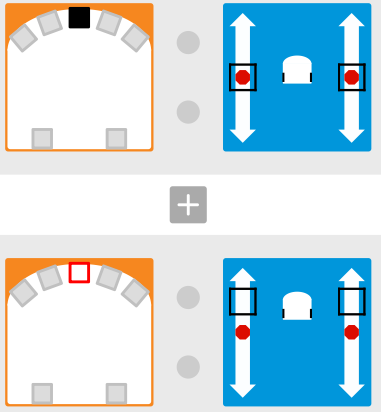
\includegraphics[width=.4\textwidth]{likes-forward}}
	\ffigbox
	{\caption{A bulldozer with tracks}\label{fig.bull}}
	{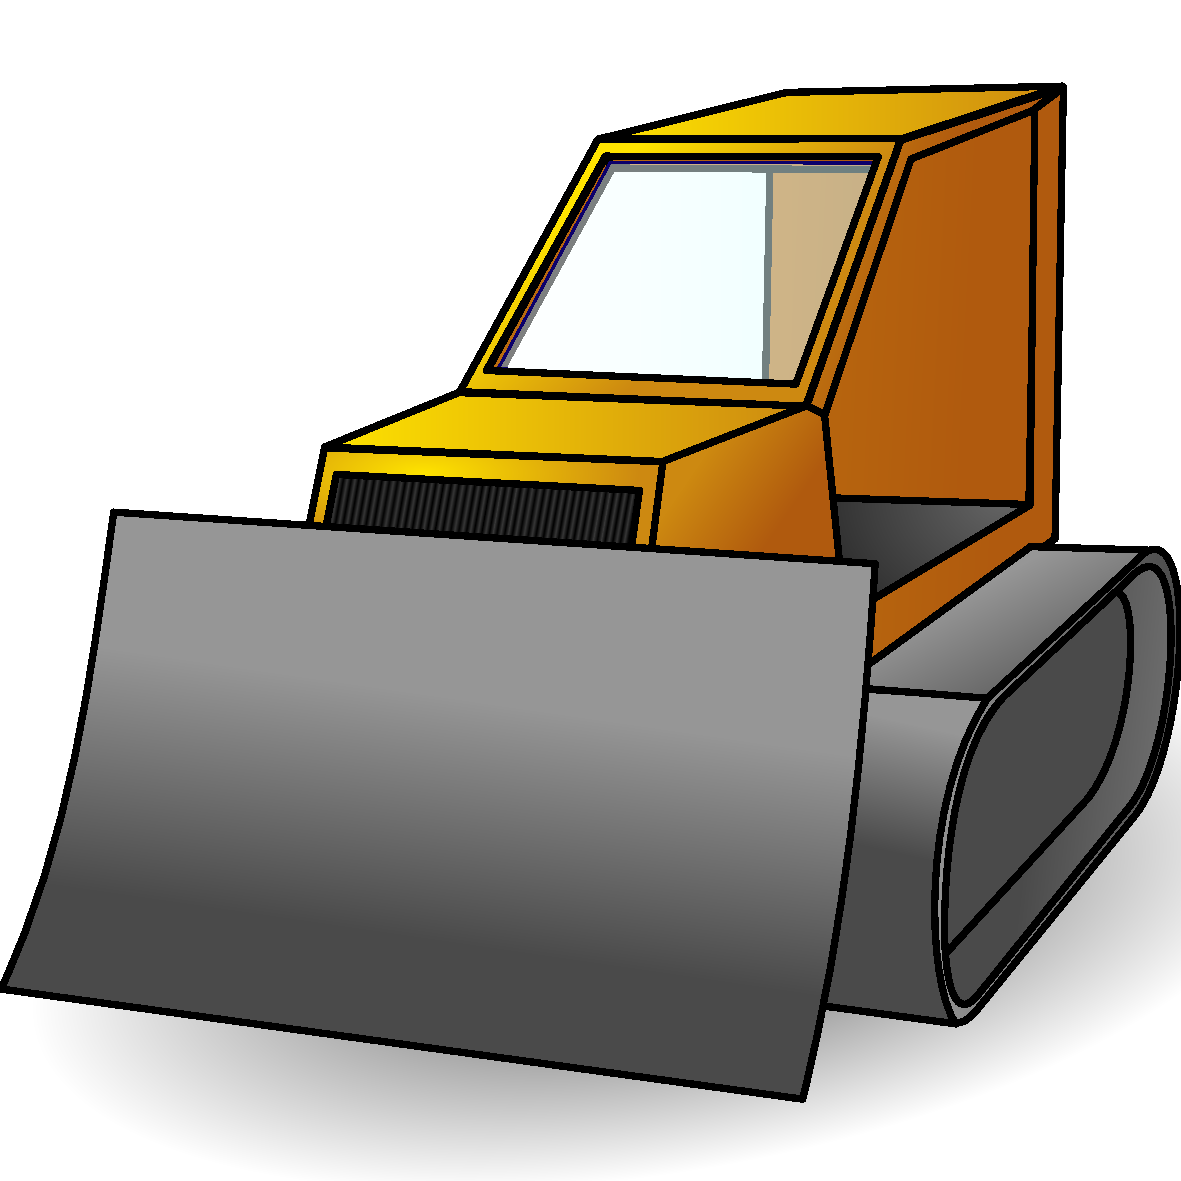
\includegraphics[width=.35\textwidth]{bulldozer}}
\end{floatrow}
\end{figure}


\sect{Steering the Thymio robot}

The Thymio robot does not have a steering wheel like a car or a
handlebar like a bicycle. So how can it turn? The robot uses
\emph{differential drive}, which is familiar from tracked vehicles like the
bulldozer (\cref{fig.bull}). Instead of turning a handlebar a
desired direction, the left and right tracks or wheels are driven by
individual motors at \emph{different} speeds. If the right track moves
faster than the left one, the vehicle turns left, and if the left track
moves faster than the right one, the vehicle turns right.

In VPL you can implement differential drive on the Thymio robot by
setting the left and right sliders of a motor action block, and therefore the wheel speeds, to
different values.
The greater the difference between the speeds, the tighter the turn. To
achieve a large difference of speeds, you can drive one track forward
and one track backwards. In fact, if one track moves forward at a
certain speed, while the other track moves backwards at the \emph{same}
speed, the Thymio turns in place.
For instance, in the motor action block \blksm{differential}, the left slider has
been set for fast speed backwards, while the right slider has been set
for fast speed forwards.
The result is that the robot will turn to the left, as indicated by the small image of the robot.

Experiment with an event-action pair such as: \blkc{turning}

Set the left and right sliders, run the program
and touch the center button; to stop the robot click on \blksm{stop}.
Now you can change the sliders and try again.

\trickbox{The icon of Thymio in the center of the motor action block shows an animation of the movement of the robot when you move the sliders.}


\sect{The robot likes you}

A real pet follows you around. To make the robot follow your hand, add
two additional event-action pairs: if the robot detects an object in
front of its left-most sensor, it turns to the left, while if it detects
an object in front of its right-most sensor, it turns to the right.

{\raggedleft \hfill Program file \bu{likes.aesl}}

The program for the robot that likes you consists of two event-action pairs, as shown in \cref{fig.likes}.
Experiment with the sliders on each motor action block.

\begin{figure}
	\subfigure[The robot likes you]{
		\label{fig.likes}
		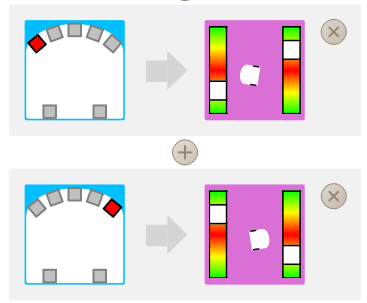
\includegraphics[width=.4\textwidth]{likes-turns}
	}
	\hfill
	\subfigure[The robot doesn't like you]{
		\label{fig.hates}
		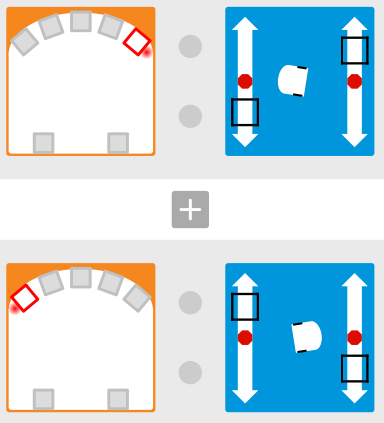
\includegraphics[width=.4\textwidth]{hates}
	}
	\caption{Programs for pet robot}
\end{figure}

\exercisebox{\thechapter.1}{
Modify the behaviour of the pet robot so that it starts moving forward when the program
is run and stops when it detects the edge of a table (or a strip of black tape).}

As explained in \cref{ch.moving}, a lot of light will be reflected
from a white surface, while very little light will be reflected from a
black surface.
You will have to experiment with the horizontal sensor block to determine when to click on a white square and when on a red square, depending on the floor or table where you place the robot.


\exercisebox{\thechapter.2}{
What happens if you change the order of
the event-action pairs that you used in the previous exercise?
}


\sect{The robot doesn't like you}

Sometimes your pet may be in a bad mood and turn away from your hand.
Write a program that causes this behavior in the robot.

{\raggedleft \hfill Program file \bu{does-not-like.aesl}}

Open the program for the pet that likes you and exchange the association
of the events with the actions. Detection of an obstacle by the left
sensor causes the robot to turn right, while detection of an obstacle by
the right sensor causes the robot to turn left, as shown in \cref{fig.hates}.

% \begin{figure}[htb]
% \begin{center}
% \gr{hates}{0.4}
% \caption{The robot doesn't you}\label{fig.hates}
% \end{center}
% \end{figure}

\exercisebox{\thechapter.3}
{
Experiment with the sensors.
The front horizontal sensors are numbered 0, 1, 2, 3, 4 from the left of the robot to its right.
The rear sensors are numbered 5 for the left one and 6 for the right one.
Instead of using sensors 0 and 4 as before:
\begin{itemize}[noitemsep,nosep,leftmargin=*]
\item Use sensors 1 and 3 to turn the robot left and right,
respectively.
\item Use both sensors 0 and 1 to turn the robot left and both sensors 3
and 4 to turn the robot right.
\item Add event-action pairs for the rear sensors 5 and 6.
\end{itemize}
}

\sect{Setting the sliders precisely (advanced)}

It is difficult to set the sliders precisely so that, for example, both
motors run at the same speed. By looking at the translation of the
event-action pairs into a textual program you can improve the precision.
\Cref{fig.textcode} shows the program where the pet likes you and follows you around along with the text translation at the right of the VPL window.
This text is modified automatically when you edit the event-action pairs.

\begin{figure}
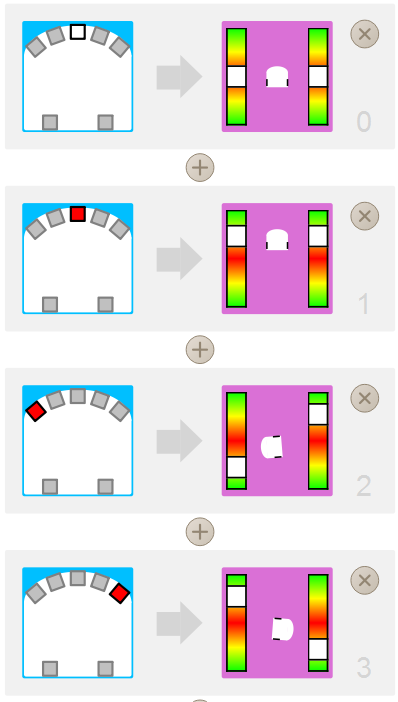
\includegraphics[width=0.3\textwidth]{follow4}
\hfill
\begin{minipage}[b]{0.6\textwidth}
\footnotesize
\begin{lstlisting}
onevent prox
	if prox.horizontal[2] < 400 then
		motor.left.target = 0
		motor.right.target = 0
	end
	if prox.horizontal[2] > 500 then
		motor.left.target = 300
		motor.right.target = 300
	end
	if prox.horizontal[0] > 500 then
		motor.left.target = -300
		motor.right.target = 300
	end
	if prox.horizontal[4] > 500 then
		motor.left.target = 300
		motor.right.target = -300
	end
\end{lstlisting}
\end{minipage}
\caption{A VPL program and the corresponding text program.}
\label{fig.textcode}
\end{figure}

The line \p{onevent prox} means: whenever the event of sampling the
horizontal distance sensors (the \emph{proximity} sensors, abbreviated \emph{prox}) occurs (it
occurs 10 times a second), the lines that follow will be run.

When the event happens, Thymio checks the values of the sensors using a condition of type \p{if} \ldots \ \p{then} \ldots \ \p{end}.
It starts by testing the sensor number 2 (front center) as we see from \p{prox.horizontal[2]}.
If this value is lower than 400, then Thymio sets the speeds of the left and right motors to 0 using the statements \p{motor.left.target = 0} and \p{motor.right.target = 0}.
Every \p{if} \ldots \ \p{then} \ldots \ \p{end} block tests a specific sensor and executes or not the associated action, as a function of the result of the test.
Hence it corresponds to an event-action pair:
\begin{enumerate}[start=0,noitemsep,nosep]
	\item tests if nothing is in front ; if that is true, Thymio stops.
	\item tests if something is in front ; if that is true, Thymio goes forward.
	\item tests if there is something at left ; if that is true, Thymio turns left.
	\item tests if there is something at right ; if that is true, Thymio turns right.
\end{enumerate}
Finally, once the Thymio has read all these sensors, it waits for the next event \p{prox} and starts these tests again, indefinitely.

To write programs in text mode, use the AsebaStudio environment (\cref{ch.next}).

\trickbox{By moving the sliders on the motor action blocks, you will
see that the target speeds of the motors (\p{moter.X.target}) jump by steps of 50 in the range $-$500
to 500.
By moving the sliders carefully, you can set the speeds to any of these values.
}